%%%%%%%%%%%%%%%%%%%%% chapter.tex %%%%%%%%%%%%%%%%%%%%%%%%%%%%%%%%%
%
% sample chapter
%
% Use this file as a template for your own input.
%
%%%%%%%%%%%%%%%%%%%%%%%% Springer-Verlag %%%%%%%%%%%%%%%%%%%%%%%%%%

\chapter{Unsupervised Learning and clustering}
\section{Vantaggi dell' Unsupervised Learning}
%Fino ad ora abbiamo assunto che i campioni di training utilizzati per progettare un classificatore sono stati etichettati in base alla classe di appartenenza. Le procedure che utilizzano campioni etichettati sono detti \emph{supervised}. Adesso verranno analizzate un numero di procedure \emph{unseupervised}, le quali usano campioni non etichettati, quindi non abbiamo una conoscenza del loro stato della natura. Ci sono cinque ragioni di base per cui si potrebbe essere interessati ad una procedura \emph{unsupervised}. Primo, collezionare ed etichettare un grande numero di campioni potrebbe risultare molto costoso. Per esempio, registrare le voci è semplice, ma un etichettatura del parlato - quindi segnare quale parola o fonema è stato pronunciato per ogni istante - può essere molto costoso in termini di tempo. Se un classificatore potrebbe essere crudelmente progettato su un piccolo insieme di campioni etichettati e poi metterlo appunto permettendogli di essere eseguito senza supervisione su un grande insieme di campioni non etichettati, molto tempo e problemi possono essere evitati. Secondo, si potrebbe pensare di procedere al contrario: addestrare un grande numero di dati non etichettati e poi usare un metodo per etichettare i gruppi (\emph{cluster}) di dati trovati.Questo è il tipico funzionamento di un applicazione di \emph{data mining}, dove i contenuti di un grande database non sono conosciuti in anticipo. Terzo, in molte applicazioni le caratteristiche dei pattern possono cambiare molto lentamente nel tempo, per esempio in un classificatore di alimenti le cose potrebbero cambiare in base alle stagioni. Se questi cambiamenti possono essere rilevati dal classificatore eseguendolo in modo \emph{unsupervised}. Quarto, possiamo usare i metodi \emph{unsupervised} per trovare della \emph{feature} che saranno utili poi per la classificazione. Infine, nella fase iniziale di investigazione dei dati potrebbe essere utile per eseguire un analisi esplorative dei dati ottenendo la comprensione della natura o della struttura dei dati. La scoperta di sottoclassi distinte - \emph{cluster} i cui membri sono molto simili l'uno con l'altro - o grandi distanze tra le caratteristiche attese potrebbero suggerirci che altera in modo significativo l'approccio di progettare il classificatore. \\
%Dovremmo incominciare con delle assunzioni molto restrittive, quindi che la forma delle distribuzioni di probabilità sono conosciute e l'unica cosa che deve essere addestrata sono i valori sconosciuti del vettore dei parametri. \'E abbastanza interessante notare che la soluzione formale di questo problema si rivelerà essere abbastanza identica al problema affrontato per il caso \emph{supervised} nel cap. \ref{tecnicheParametriche}.\\

Fino ad ora abbiamo assunto che i campioni di training utilizzati per progettare un classificatore sono stati etichettati in base alla classe di appartenenza. Quindi si ha a disposizione un insieme di dati dei quali conosciamo la loro natura di appartenenza. Le procedure che operano su quest'insieme di dati sono dette \emph{unsupervised}. Questa modalità è utilizzata per una serie di ragioni. Esempio, raccogliere ed etichettare un gran numero di campioni può risultare molto costoso, in alcuni casi potrebbe essere non fattibile in quanto non si ha a disposizione un esperto. Inoltre da un punto di vista statistico è più facile affrontare il problema nel caso non supervisionato che nel caso supervisionato, nel senso che è molto difficile etichettare i campioni da parte di un esperto che molto spesso lo riesce a fare soltanto per un numero di campioni molto ridotto, problema invece che non si ha nel caso \emph{unsupervised} in quanto il numero di campioni non etichettato può anche crescere a dismisura dato che non è vincolato dal lavoro ulteriore di un esperto che etichetta i campioni. Quindi dal punto di vista statistico la rappresentatività dei dati non etichettati, tipicamente è maggiore dei dati etichettati, inoltre i metodi non supervisionati possono essere utilizzati anche per l'estrazione di caratteristiche. 
Un esempio è quando non si conosce la sorgente dei dati, tipicamente i dati vengono raccolti da sensori e non si ha neanche un esperto che riesce ad etichettare i dati (\emph{fetaure}), quindi l'approccio non supervisionato oltre ad apparire come un approccio per la classificazione di dati non etichettati  potrebbe apparire anche come un processo di preelabrazione dei dati. Per esempio quando si ha a disposizione una quantità enorme di dati, questi vengono analizzati con la condizione che non si sa da dove derivano e quale è l'etichetta. Quindi si ha a disposizione  molti campioni per effettuare un analisi statistica dei dati senza l'ausilio degli esperti, questo processo produce un insieme ridotto delle osservazioni e sono queste quelle che verranno poi sottoposte all'analisi. Sotto questo aspetto Il processo di classificazione non supervisionato non è un processo di classificazione ma un processo di estrazione di carattaristiche. Le tecniche che verranno utilizzate, sono tecniche di \emph{data mining} (investigare i dati). L'analisi dei dati per esplorazione (mining) può risultare utile alla comprensione della natura e struttura dei dati, quindi solo dopo aver effettuato un esplorazione attenta dei dati è possibile analizzarli e quindi sarà possibile poi dire si i dati analizzati corrispondono ad un determinato processo.\\

\section{Introduzione}
Stiamo nel caso in cui l'apprendimento è non supervisionato, quindi il caso in cui i campioni che abbiamo a disposizione non sono etichettati. \'E un caso abbastanza generale poiché è molto difficile raccogliere ed etichettare un gran numero di campioni, in quanto effettuare tali operazioni è costoso in termini di tempo, ma soprattutto è costoso in termini di energie di esperti del settore spese per poter operare un etichettatura dei campioni. Quindi in alcuni casi abbiamo una raccolta di dati, anche abbastanza considerevole, non etichettati però rappresentativi di fenomeni abbastanza complessi che devono essere studiati. Studiare un fenomeno non significa soltanto riuscire a determinare la struttura, ma molto spesso significa proprio rilevare eventi che non sono noti, rilevare anomalie che rappresentano eventi significativi, per cui scoprire caratteristiche dai dati è l'obiettivo dell'unsupervised learning. Il termine apprendimento è legato al fatto che i parametri delle distribuzioni di probabilità dei modelli non sono noti e bisogna renderli noti soltanto dopo una fase di addestramento di un sistema che si va a progettate. Per prima cosa si dovrebbe progettare un sistema di classificazione assumendo che si basi sul criterio MAP, quindi la probabilità a posteriori segue la regola di Bayes, però le probabilità che entrano in gioco nella regola di Bayes non sono note, non sono note le proprietà a priori ed in particolare le probabilità condizionate ovvero la verosomiglianza e di conseguenza se non sono note queste non è nota neanche l'evidenza, ovvero il denominatore della regola di Bayes, quindi di conseguenza non è nota la probabilità a posteriori. L'ipotesi in questo caso, come abbiamo già fatto per l'apprendimento supervisionato è quella di avere la conoscenza del modello, cioè di avere conoscenza della distribuzione di probabilità dei dati. \'E un ipotesi forte in quanto ci appelliamo al teorema del limite centrale il quale dice che su un numero di campioni infinito le distribuzioni di probabilità tendono ad essere gaussiane, ci limitiamo pertanto a stimare o meglio ad apprendere i parametri delle distribuzioni di probablità gaussiane, che  nella maggior parte dei casi sono gaussiane multivariate caratterizzate da una media e da una matrice di covarianza. Un punto essenziale è come scoprire le regolarità dei dati, cioè se i dati che io raccolgo si comportano in modo regolare, dal punto di vista matematico regolare significa che è possibile interpolare questi dati attraverso delle funzioni matematiche che appaiono funzioni regolari, quindi scoprire le regolarità vuol dire scoprire un modello di comportamento che è assolutamente importante per il rilevamento di anomalie. Praticamente a cosa serve la teoria non supervisionata ed il clustering? Immaginiamo di avere una raccolta di dati considerevole, etichettare questi dati è improponibile, avere conoscenza di cosa corrispondono questi dati è altrettanto improponibile allora l'esperto non lo si chiama proprio, non viene proprio interpellato per guardare i dati, si fa una scrematura, ovvero una pulizia dei dati, quindi si studiano le regolarità dei dati attraverso le tecniche di unsupervised learning o clustering in modo tale che i prototipi dei cluster che poi vengono identificati (il raggruppamento) verranno poi posti all'attenzione degli esperti, cioè quindi non i dati stessi ma i prototipi dei cluster i cui ho suddiviso i dati, naturalmente i prototipi dei cluster in cui ho suddiviso i dati sarà in numero nettamente minore dei dati da osservare e quindi porta ad una realizzazione del procedimento di etichettatura da parte di un esperto. Pertanto quello che stiamo dicendo è che molto spesso l'apprendimento non supervisionato è una fase di elaborazione, cioè quella fase di analisi dei dati che viene prima di una analisi più attenta dei dati stessi. Quindi ad un procedimento non supervisionato quasi sempre segue un procedimento supervisionato. In alcuni casi però è possibile anche che il risultato di un apprendimento non supervisionato sia già sufficiente per la comprensione del dataset e quindi l'esperto non viene interpellato. Quando i pattern appaiano molto densi allora il clusetring risulta essere molto agevole, quindi questa procedura è molto utile quando di dati sono densamente distribuiti intorno ad un prototipo o centroide. Quando invece i dati si distribuiscono in modo non così denso intorno ad un centroide allora è molto più difficile determinare i centroidi, è anche molto più difficile determinare i veri cluster e quindi è necessaria una fase di etichettatura. L'apprendimento non supervisionato rappresenta una grossolana suddivisione dei dati in gruppi. Il problema va però affrontato in un modo formalmente corretto.

\section{Mixture Densities and Identifiability}
Cominciamo con l'assunzione che conosciamo la completa struttura probabilistica del problema, con la sola eccezione di non conoscere i valori di alcuni parametri. Per essere più specifici, facciamo le seguenti assunzioni:

\begin{enumerate}
\item I campioni provengono un numero di $c$ classi che conosciamo
\item Le probabilità a priori $P(\omega_j)$ per ogni classe $j=1, \dots, c$ sono conosciute
\item Le densità di probabilità sono conosciute $p(\mathbf{x}|\omega_j , \mathbf{\Theta}_j)$
\item Valori dei vettori dei parametri $\mathbf{\Theta}_1, \dots, \mathbf{\Theta}_c$ sono sconosciuti
\item Le etichette per ogni categoria sono sconosciute
\end{enumerate}
A differenza dello studio effettuato nell'apprendimento supervisionato che veniva effettuato per classi, qui non conosciamo le classi di appartenenza, e quindi deve essere fatto su tutti i dati ipotizzando che i dati provengono da $c$ classi. Ma non sappiamo quali sono le classi perchè i pattern non sono etichettati. Si ipotizza che la distribuzione di probabiltà non è altro che una combinazione lineare delle distribuzioni di probabilità delle singole classi che però non sono note. Immagino che i dati provengono da $c$ classi, non si è a conoscenza di quali sono le classi, ma si sa  soltanto che la distribuzione di probabilità per ogni classe è per esempio una gaussiana multivariata, di cui non conosco ne la media ne la matrice di covarianza per ogni classe. Naturalmente poiché i dati non sono etichettati non posso fare un analisi per classe, ma devo fare un analisi di tutti i dati. Allora immagino che la distribuzione di probabilità totale dei dati non è altro che una combinazione lineare della distribuzione di probabilità per ogni singola classe, che prende il nome di mixtura di densità di probabilità, che nel caso di gaussiane prende il nome di mixture di gaussiame (MOG). L'evidenza $p(\mathbf{x})$, cioè la distribuzione di probabilità di un pattern qualsiasi $\mathbf{x}$ indipendentemente  da quale classe apparitene non è altro che la probabilità marginale delle probabilità congiunte. Posso certamente dire che 
\begin{equation}\label{93}
p(\mathbf{x}) = \sum_{j=1}^c p(\mathbf{x}, \omega_j)
\end{equation}
questa non è altro che la distribuzione di probabilità marginale della distribuzione di probabilità congiunta di $p(\mathbf{x}, \omega_j)$, ricordando che per la distribuzione di probabilità congiunta (la tabella a doppia entrata) la probabilità marginale si calcola per colonne o per righe. La \ref{93} è possibile riscriverla come
\begin{equation}
p(\mathbf{x}) = \sum_{j=1}^c p(\mathbf{x}|\omega_j) P(\omega_j)
\end{equation}

\noindent Assumiamo che i campioni sono stati ottenuti selezionando lo stato della natura $\omega_j$ con probabilità $P(\omega_j)$ e poi selezionando un osservazione $\mathbf{x}$ in accordo con la distribuzione di probabilità $p(\mathbf{x}|\omega_j, \mathbf{\Theta}_j)$. Così, la densità di probabilità per i campioni è data da
\begin{equation}
p(\mathbf{x}|\mathbf{\Theta}) = \sum_{j=1}^c p(\mathbf{x}|\omega_j, \mathbf{\Theta}_j) P(\omega_j)
\end{equation}
dove $\mathbf{\Theta} = (\mathbf{\Theta_1}, \dots, \mathbf{\Theta}_c)^t$, non è altro un vettore di vettori di parametri. Quindi ogni $\mathbf{\Theta}_j$ è un vettore di parametri, per fare un esempio nel caso di una gaussiana $\mathbf{\Theta}_j$ non è altro che il vettore costituito da media e matrice di covarianza della $j$-esima distribuzione gaussiana multivariata. Per ovvie ragioni, la funzione di densità in questa forma è chiamata \emph{mixture density}, le distribuzioni di probabilità condizionate sono chiamate \emph{component density} e le probabilità a priori sono chiamate \emph{mixing parameters}. L'obiettivo base sarà quello di usare i campioni che seguono la \emph{mixture density} per stimare il vettore parametri sconosciuti $\mathbf{\Theta}$.  Se l' obiettivo è la classificazione allora una volta trovato $\mathbf{\Theta}$ possiamo decomporre la mixtura in tante componenti e usare un classificatore MAP (\emph{maximum a posteriori}) sulle densità derivate. Prima di cercare una soluzione a questo problema, ci chiediamo comunque se è possibile o meno ricavare $\mathbf{\Theta}$ dalle mixture. Supponiamo che abbiamo un illimitato numero di campioni e che usiamo un metodo non parametrico della sezione \ref{metodinonparametrici} per determinare il valore di $p(\mathbf{x}|\mathbf{\Theta})$ per ogni $\mathbf{x}$. Se c'è un solo valore di $\mathbf{\Theta}$ che sarà prodotto dai valori osservati per $p(\mathbf{x}|\mathbf{\Theta})$, allora la soluzione è possibile in linea si principio, invece se molti valori di $\mathbf{\Theta}$ possono produrre gli stessi valori per $p(\mathbf{x}|\mathbf{\Theta})$, allora non ci sono speranze di ottenere una soluzione unica.\\
Queste considerazioni   ci portano alla seguente definizione: Una funzione di densità $p(\mathbf{x}|\mathbf{\Theta})$ è detta \emph{identificabile} se $\mathbf{\Theta} \neq \mathbf{\Theta}'$ implica che esiste un $\mathbf{x}$ tale che $p(\mathbf{x}|\mathbf{\Theta}) \neq p(\mathbf{x}|\mathbf{\Theta}')$, questo significa che quando si stimano i $\mathbf{\Theta}$ si potrebbe ottenere per differenti valori di $\mathbf{\Theta}$ la stessa distribuzione di probabilità, cosa che non deve accadere altrimenti il procedimento non va a buon termine.
Facciamo un semlice esempio dove si considera il caso in cui $x$ è binario (quindi può assumere $0$ o $1$) e $P(x|\mathbf{\Theta})$ è una mixtura di due binomiali
\begin{equation}
\begin{split}
P(x|\mathbf{\Theta}) &= \frac{1}{2} \Theta_1^x(1-\Theta_1)^{1-x} + \frac{1}{2}\Theta_2^x(1-\Theta_2)^{1-x}\\
&= \begin{cases}
\frac{1}{2}(\Theta_1 + \Theta_2) & \text{se} \ x =1\\
1 - \frac{1}{2}(\Theta_1 + \Theta_2) & \text{se} \ x = 0 
\end{cases} 
\end{split}
\end{equation}
\'E identificabile questa mixtura di densità? Presi due valori $\mathbf{\Theta}$ e $\mathbf{\Theta}'$ che sono diversi, esiste almeno un $x$ per cui $P(x|\mathbf{\Theta}) \neq P(x|\mathbf{\Theta}')$? \\
Supponiamo, per esempio, che conosciamo il valore di $P(x=1|\mathbf{\Theta}) = 0.6$ e quindi che $P(x=0|\mathbf{\Theta}) = 0.4$. Conosciamo la funzione $P(x|\mathbf{\Theta})$, ma non possiamo determinare $\mathbf{\Theta}$ e quindi non possiamo estrarre le componenti della distribuzione. Inoltre possiamo dire che $\Theta_1 + \Theta_2 = 1.2$. Come potremmo mai trovare dei valori $\Theta_1$ e $\Theta_2$ che identificano in modo inequivocabile la densità di probabilità se praticamente la loro somma in entrambi i casi è sempre uguae ad $1.2$? \\
Quindi è impossibile trovare una combinazione di parametri che sia identificabile.
Così, abbiamo un caso per il quale la distribuzione di mixture è completamente non identificabile, un caso per il quale la tecnica \emph{unseupervised} non può essere applicata in linea di principio. Questo tipo di problema si presenta comunemente nel caso di dati discreti, la presenza di molte componenti potrebbe rendere il problema abbastanza difficile, invece nel caso continuo, il problema è meno severo. \'E possibile mostrare che la mixtura di distribuzioni normali (mixtura di gaussiane) sono generalmente identificabili e i parametri di una semplice mixtura sono
\begin{equation}
p(x|\mathbf{\Theta}) = \frac{P(\omega_1)}{\sqrt{2\pi}} \exp \left[ -\frac{1}{2}(x-\Theta_1)^2 \right] + \frac{P(\omega_2)}{\sqrt{2\pi}} \exp \left[ -\frac{1}{2}(x-\Theta_2)^2 \right] 
\end{equation}
questa mixtura non può essere unicamente identificata se $P(\omega_1) = P(\omega_2)$, dato che $\Theta_1$ e $\Theta_2$ possono essere intercambiate senza cambiare $p(x|\mathbf{\Theta})$.

\section{Maximum Likelihood estimates}
Dato un insieme $\mathcal{D}= \{\mathbf{x}, \dots, \mathbf{x}_n \}$ composto da $n$ campioni, immaginiamo $n$ che sia infinito o comunque molto alto, i vettori sono \emph{i.i.d.}, dobbiamo inoltre ricordare che i campioni non sono etichettati e la mixtura di densità è
\begin{equation}
p(\mathbf{x}|\mathbf{\Theta}) = \sum_{j=1}^c p(\mathbf{x}|\omega_j, \mathbf{\Theta}_j) P(\omega_j)
\end{equation}
dove tutti i parametri del vettore $\mathbf{\theta}$ sono fissati ma non conosciuti. Conosciamo la provenienza dei dati ma non conosciamo ogni campione da quale classe proviene. Inoltre facciamo un altra ipotesi, che ogni classe ha un modello di distribuzione di probabilità noto, quindi possiamo immaginare che siano tutte gaussiane delle quali però non conosciamo le medie e le matrici di covarianza. L'obiettivo è quello di stimare i parametri di queste distribuzioni di probabiità, quindi di classi che non conosciamo la suddivisione. Allora non lavoriamo sul termine a destra perchè anche se diciamo che sono gaussiane non possiamo lavorare su media e covarianza di gruppi di dati che non conosco l'etichettatura, quindi si deve necessariamente lavorare sul termine a sinistra $P(\mathbf{x}|\mathbf{\Theta})$ augurandosi di poter fare qualche cosa anche sul termine a destra. Quindi $\mathbf{\Theta}$ è fisso ma non è noto, fisso significa che non cambia, è indipendentemente dal numero dei dati, una cosa poco relistica.\\
La verosomiglianza (\emph{likelihood}) dei campioni osservati è, per definizione, la probabilità congiunta
\begin{equation}
p(\mathcal{D}|\mathbf{\Theta})  =\prod_{k=1}^n p(\mathbf{x}_k|\mathbf{\Theta})
\end{equation}
$P(\mathcal{D}|\mathbf{\Theta})$ è la probabilità di tutto il training set dato $\mathbf{\Theta}$, ma abbiamo detto che  $\mathcal{D}= \{\mathbf{x}, \dots, \mathbf{x}_n \}$ ed essendo \emph{i.i.d.} posso scrivere $P(\mathcal{D}|\mathbf{\Theta})$ come produttoria. Dobbiamo trovare $\mathbf{\Theta}$, che in questo caso è il vettore dei parametri di tutti i parametri di tutte le classi, quindi tutte le medie e le covarianze di tutte le classi $c$ che ho a disposizione. Stiamo lavorando sul tutto il training set e non soltanto su una classe. L'obiettivo è massimizzare $p(\mathcal{D}|\mathbf{\Theta})$, quindi bisogna trovare il valore di $\mathbf{\hat{\Theta}}$ che sostituito nella distribuzione d probabilità $P(\mathcal{D}|\mathbf{\Theta})$ rendono più verosimile  
la distribuzione di probabilità a quella che è la reale distribuzione di probabilità, quindi una stima a massima verosomiglianza. La stima a massima verosomiglianza  di $\mathbf{\hat{\Theta}}$ è proprio il valore di $\mathbf{\Theta}$ che massimizza $p(\mathcal{D}|\mathbf{\Theta})$.\\
Per massimizzare una funzione facciamo la derivata e si pone uguale a zero. In particolare se i parametri $\mathbf{\Theta}$ sono tanti, in questo caso sono $c$ vettori di parametrim, allora bisogna fare $kc$ derivate parziali dove $k$ è il numero di parametri per la distribuzione e nel caso gausiano $k=2$. 
Se assumiamo che $p(\mathcal{D}|\mathbf{\Theta})$ è una funzione differenziabile di $\mathbf{\Theta}$, allora è possibile dedurre alcune necessarie ed interessanti condizioni per $\mathbf{\hat{\Theta}}$. Dato $l$ il logaritmo della verosomiglianza, e dato $\mathbf{\nabla}_{\mathbf{\theta}_1}l$ il gradiente di $l$ rispetto a $\mathbf{\Theta}_i$, allora
\begin{equation}
l= \sum_{k=1}^n \ln p(\mathbf{x}_k|\mathbf{\Theta})
\end{equation}
e
\begin{equation}
\mathbf{\nabla_{\Theta_i}} l = \sum_{k=1}^n \frac{1}{p(\mathbf{x}_k|\mathbf{\Theta})} \mathbf{\nabla_{\Theta_i}} \left[ \sum_{j=1}^c p(\mathbf{x}_k| \omega_j, \mathbf{\Theta}_j) P(\omega_j) \right]
\end{equation}
Inoltre assumiamo che gil elementi di $\mathbf{\Theta}_i$ e $\mathbf{\Theta}_j$ sono indipendenti soltanto se $i \neq j$, e introducendo la probabilità a posteriori che è uguale a
\begin{equation}
P(\omega_i|\mathbf{x}_k, \mathbf{\Theta}) = \frac{p(\mathbf{x}_k|\omega_i, \mathbf{\Theta}_i)P(\omega_i)}{p(\mathbf{x}_k|\mathbf{\Theta})}
\end{equation}
osserviamo che il gradiente della $log-likelihood$ può essere riscritto in una forma interessante
\begin{equation}
\mathbf{\nabla_{\Theta_i}} l = \sum_{k=1}^n P(\omega_i|\mathbf{x}_k, \mathbf{\Theta}) \mathbf{\nabla_{\mathbf{\Theta}_i}} \ln p(\mathbf{x}_k|\omega_i, \mathbf{\Theta}_i)
\end{equation}
Poichè il gradiente deve svanire al valore di $\mathbf{\Theta}_i$ che massimizza $l$, la stima a massima verosomiglianza $\mathbf{\hat{\Theta}}_i$ deve soddisfare le condizioni
\begin{equation}\label{8}
\sum_{k=1}^n P(\omega_i|\mathbf{x}_k, \mathbf{\hat{\Theta}}) \mathbf{\nabla_{\Theta}}_i \ln p(\mathbf{x}_k|\omega_i, \mathbf{\hat{\Theta}}_i) = 0 \quad \quad \quad i=1, \dots, c
\end{equation}
Risolvendo quest'equazione per $\mathbf{\hat{\Theta}}_i$ troveremo la soluzione della massima verosomiglianza.\\
Non è difficile generalizzare questi risultati includendo le probabilità a priori $P(\omega_i)$ tra le quantità sconosciute. In questo caso del valore che massimizza $p(\mathcal{D|\mathbf{\Theta}})$
si estende su $\mathbf{\Theta}$ e $p(\omega_i)$, soggetti ad i seguenti vincoli
\begin{equation}
P(\omega_i) \geq 0 \quad \quad \quad i=1, \dots, c
\end{equation}
e
\begin{equation}
\sum_{i=1}^c P(\omega_i)  = 1 
\end{equation}
Denotiamo con $\hat{P}(\omega_i)$ la stima a massima verosomiglianza per $P(\omega_i)$, e denotiamo dato $\mathbf{\hat{\Theta}}_i$ la stima a massima verosomigliaza per $\mathbf{\Theta}_i$. \'E possibile dimostrare che se la funzione di verosomiglianza è differenziabile e se $\hat{p(\omega_i)\neq 0}$ per qualsiasi $i$, allora $\hat{P}(\omega_i)$ e $\mathbf{\hat{\Theta}}$ deve soddisfare
\begin{equation}\label{11}
\hat{P}(\omega_i) = \frac{1}{n} \sum_{k=1}^n \hat{P}(\omega_i | \mathbf{x}_k, \mathbf{\hat{\Theta}})
\end{equation}
e
\begin{equation}\label{12}
\sum_{k=1}^n \hat{P}(\omega_i|\mathbf{x}_k, \mathbf{\hat{\Theta}}) \mathbf{\nabla_{\mathbf{\Theta}_i}} \ln p(\mathbf{x}_k|\omega_i, \mathbf{\hat{\Theta}}_i) = 0
\end{equation}
dove
\begin{equation}\label{13}
\hat{P}(\omega_i|\mathbf{x}_k, \mathbf{\hat{\Theta}}) = \frac{p(\mathbf{x}_k|\omega_i, \mathbf{\hat{\Theta}}_i)\hat{P}(\omega_i)}{\sum_{j=1}^c p(\mathbf{x}_k|\omega_j, \mathbf{\hat{\Theta}}_j)\hat{P}(\omega_j)}
\end{equation}
Queste equazioni hanno la seguente interpretazione. L'equazione \ref{11} ci dice che la stima a massima verosomiglianza della probabilità di una categoria è la media su tutto l'intero dataset delle stime derivate da ogni campione - ogni campione è ugualmente pesato. L'equazione \ref{13} è correlata al teorema di Bayes, ma da notare che il numeratore dipende da $\mathbf{\hat{\Theta}}_i$ e non su tutti i $\mathbf{\hat{\Theta}}$.

\section{Application To Normal Mixtures}
\'E istruttivo vedere come questi risultati si applicano al caso in cui le distribuzioni sono gaussiane multivariate, $P(\mathbf{x}|\omega_i, \mathbf{\Theta}_i)\sim N(\mathbf{\mu}_i, \mathbf{\Sigma}_i)$. La tabella seguente illustra i casi che potrebbero verificarsi indicando con $(\times)$ i parametri conosciuti e con $(?)$ i parametri non conosciuti:

\begin{table}[ht]
\centering
\begin{tabular}{l cccccccccc}
\hline
Case & $\mathbf{\mu}_i$  & $\mathbf{\Sigma}_i$ & $\mathbf{P(\omega_i)}$ & $c$\\
\hline
 1 &  $?$  & $\times$  &    $\times$   &  $\times$  \\
 2 & $?$ & $?$ & $?$ &    $\times$   \\
 3 & $?$ & $?$ & $?$ & $?$ \\
\hline
\end{tabular}
\end{table}
\noindent Il caso 1 è il più semplice ed è quello che verra considerato in dettaglio. Il caso 2 è quello più realistico, mentre il terzo caso rappresenta il problema di quando ci troviamo di fronte quando tutti i dati sono completamente sconosciuti,purtroppo non è possibile risolvere il problema con la tecnica a massima verosomiglianza. 

\subsection{Case 1: Vettore media non conosciuto}
\'E noto tutto tranne la media, quindi l'unico parametro da stimare è $\mathbf{\mu}_i$, e naturalmente $\mathbf{\mu}_i = \mathbf{\Theta}_i$. Allora la verosomiglianza diventa $p(\mathbf{x}|\omega_i, \mathbf{\mu}_i)$ e la log-verosomiglianza, ovvero il logaritmo è
\begin{equation}
\ln p(\mathbf{x}|\omega_i, \mathbf{\mu}_i) = - \ln \left[ (2\pi)^{d/2} \abs{\mathbf{\Sigma}}^{1/2} \right] - \frac{1}{2}(\mathbf{x}-\mathbf{\mu}_i)' \mathbf{\Sigma}_i^{-1}(\mathbf{x}- \mathbf{\mu}_i) 
\end{equation}
adesso bisogna fare la derivata parziale rispetto a $\mathbf{\mu}_i$ allora il primo termine va a zero dato che è costante rispetto a $\mathbf{\mu}_i$, 
il secondo termine invece applicando semplici passaggi matematici otteniamo
\begin{equation}
- \frac{1}{2} \frac{(\mathbf{x}-\mathbf{\mu}_i)'(\mathbf{x}-\mathbf{\mu}_i)}{\mathbf{\Sigma}_i} = -\frac{1}{2} \frac{(\mathbf{x}-\mathbf{\mu}_i)^2}{\mathbf{\Sigma}_i}
\end{equation}
e quindi risolvendo questa semplice derivata e moltiplicando per $-1$ che è la derivata di $-\mathbf{\mu}_i$ otteniamo
\begin{equation}
\nabla_{\mu_i} \ln p(\mathbf{x}|\omega_i, \mathbf{\mu}_i) = \mathbf{\Sigma}_i^{-1}(\mathbf{x}-\mathbf{\mu}_i)
\end{equation}
una volta ottenuta la derivata allora va sostituita nella \ref{8} e va posta uguale a 0
\begin{equation}
\sum_{k=1}^n P(\omega_i|\mathbf{x}_k, \hat{\mathbf{\mu}}) \mathbf{\Sigma}^{-1}(\mathbf{x}_k - \mathbf{\hat{\mathbf{\mu}}}_i) = 0 \quad \quad \quad \text{dove} \ \ \hat{\mathbf{\mu}} = (\hat{\mathbf{\mu}}_1, \dots, \hat{\mathbf{\mu}}_c)^t
\end{equation}
da questa $\mathbf{\Sigma}_i$ è nota e quindi di conseguenza anche l'inversa $\mathbf{\Sigma}_i^{-1}$ è nota, $\mathbf{x}_k$ è noto e $\hat{\mathbf{\mu}}_i$ non è noto. Per un istante immaginiamo che $P(\omega_i|\mathbf{x}_k, \hat{\mathbf{\mu}})$ è noto, o meglio è quella probabilità aposteriori che riusciamo in modo iterativo a stimare di volta in volta, quindi ad un certo istante abbiamo una stima delle probabilità aposteriori, non abbiamo quella reale ma certamente una stima ce l'abbiamo, quindi è tra virgolette nota. Allora risolvendo rispetto a $\hat{\mathbf{\mu}}_i$ otteniamo
\begin{gather}
\sum_{k=1}^n P(\omega_i|\mathbf{x}_k, \hat{\mathbf{\mu}}) \mathbf{\Sigma}_i^{-1}(\mathbf{x}_k - \mathbf{\hat{\mathbf{\mu}}}_i) = 0\\
\sum_{k=1}^n P(\omega_i|\mathbf{x}_k, \hat{\mathbf{\mu}}) \mathbf{\Sigma}_i^{-1} \mathbf{x}_k - P(\omega_i|\mathbf{x}_k, \hat{\mathbf{\mu}}) \mathbf{\Sigma}_i^{-1} \mathbf{\hat{\mathbf{\mu}}}_i = 0\\
\sum_{k=1}^n P(\omega_i|\mathbf{x}_k, \hat{\mathbf{\mu}}) \mathbf{\Sigma}_i^{-1} \mathbf{x}_k = \sum_{k=1}^n P(\omega_i|\mathbf{x}_k, \hat{\mathbf{\mu}}) \mathbf{\Sigma}_i^{-1} \mathbf{\hat{\mathbf{\mu}}}_i \\
\mathbf{\hat{\mathbf{\mu}}}_i = \frac{\sum_{k=1}^n P(\omega_i|\mathbf{x}_k, \hat{\mathbf{\mu}}) \mathbf{\Sigma}_i^{-1} \mathbf{x}_k}{ \sum_{k=1}^n P(\omega_i|\mathbf{x}_k, \hat{\mathbf{\mu}}) \mathbf{\Sigma}_i^{-1}}
\end{gather}
$ \mathbf{\Sigma}_i^{-1}$ è nota e allora 
\begin{equation}
\mathbf{\hat{\mathbf{\mu}}}_i = \frac{\sum_{k=1}^n P(\omega_i|\mathbf{x}_k, \hat{\mathbf{\mu}})  \mathbf{x}_k}{ \sum_{k=1}^n P(\omega_i|\mathbf{x}_k, \hat{\mathbf{\mu}})}
\end{equation}
e possiamo osservare che $\mathbf{\hat{\mathbf{\mu}}}_i$ non è altro che la media ponderata degli $\mathbf{x}_k$ all'interno di una classe. Per cui,  come si può immaginare il valore di $P(\omega_i|\mathbf{x}_k, \hat{\mathbf{\mu}})$? Se sapessimo già da prima quali erano le appartenenze dei pattern ai gruppi allora era facile, bastava vedere quanti campioni stavano in ogni classe e il valore di quei campioni, quindi la porzione dei campioni che sta in una classe è $P(\omega_i|\mathbf{x}_k, \hat{\mathbf{\mu}})$. Adesso è lo stesso ragionamento, solo che poichè non conosciamo a priori quali sono le classi, ma sappiamo quante sono le classi, di volta in volta che facciamo la stima calcoliamo quanti campioni rientrano in questo gruppo, cioè fondamentalmente sommiamo i $P(\omega_i|\mathbf{x}_k, \hat{\mathbf{\mu}})$, ovvero le probabilità aposteriori che rappresentano la frazione dei campioni avente valore $\mathbf{x}_k$ e che appartengono alla $i$-esima classe sono i pesi di questa combinazione lineare e quindi della media ponderata.\\

\noindent Questo è un risultato analogo a quello che abbiamo ottenuto anche per l'apprendimento a massima verosomiglianza nel caso del supervisionato, poichè il primo caso che stiamo vedendo adesso è esattamente il primo caso nella massima verosomilianza del supervisionato, in quella situazione la media che si va a massimizzare era la media dei campioni appartenenti alla classe, quindi tutta questa base teorica per dire che il valor medio, ovvero la media della gaussiana che mi distribuisce o che modella la distribuzione dei dati di una classe la vado a calcolare semplicemente facendo la media campionaria (media dei pattern appartenenti alla classe). IN questo caso non conocsciamo quanti pattern sono in ogni classe ma è possibile stimarlo di volta in volta, e questa stima è la $P(\omega_i|\mathbf{x}_k, \hat{\mathbf{\mu}})$ che è possibile calcolare mediante la regola di Bayes 
\begin{equation}
P(\omega_i|\mathbf{x}_k, \hat{\mathbf{\mu}}) = \frac{ p(\mathbf{x}_k|\omega_i, \hat{\mathbf{\mu}}_i) P(\omega_i) }{ \sum_{j=1}^c p(\mathbf{x}|\omega_j, \hat{\mathbf{\mu}}_j) P(\omega_j)}
\end{equation}
fondamentalmente il processo è sempre iterativo, quindi abbiamo risolto il sistema di equazioni lineari, dove ne abbiamo $c$, nel caso particolare il cui il parametro da calcolare è $\mathbf{\mu}_i$. Quindi la soluzione è la media ponderata, il processo iterativo di queste stima lo facciamo lo stesso soltanto che poi ci accorgiamo che questo vettore medio ponderato cambia in virtù di quanti pattern metto nella classe (un procedimento simile al clustering k-means, parto da un centroide e di volta in volta il centroide si avvicina a quello che dovrebbe essere reale centroide del cluster ricalcolando il centroide di un cluster in modo iterativo), infatti le medie vengono calcolate in modo iterativo come 
\begin{equation}
\mathbf{\hat{\mathbf{\mu}}}_i(j+1) = \frac{\sum_{k=1}^n P(\omega_i|\mathbf{x}_k, \hat{\mathbf{\mu}}(j))  \mathbf{x}_k}{ \sum_{k=1}^n P(\omega_i|\mathbf{x}_k, \hat{\mathbf{\mu}}(j))}
\end{equation}
quindi la media al passo $j+1$ viene calcolata in virtù della media calcolata al passo $j$. Per gli informatici è un algoritmo \emph{greedy} mentre per i matematici è noto come tecnica del gradiente ascendente, ascendente perchè stiamo massimizzando la log-verosomiglianza dei dati.

\subsection{Case 2: Tutti i parametri non conosciuti}

In questo caso è noto soltanto il numero delle classi, quindi non conosciamo $P(\omega_i)$ e non conosciamo entrambi i parametri $\mathbf{\mu}_i$ e $\mathbf{\Sigma}_i$ delle gaussiane che modellano la distribuzione dei dati. Allora supponiamo che la verosomiglianza non è altro che una mixtura a due componenti
\begin{equation}
p(x|\mu, \sigma^2) =\frac{1}{2 \sqrt{2\pi} \sigma} \exp \left[ -\frac{1}{2} \left( \frac{x -\mu}{\sigma} \right)^2  \right]  + \frac{1}{2 \sqrt{2\pi}} \exp \left[ -\frac{1}{2}x^2 \right]
\end{equation}
quindi la funzione di verosomiglianza è rappresentata da questa mixtura e si nota che nella seconda si ha media pari a zero e varianza uguale ad uno (normale standardizzata). La verosomiglianza per $n$ campioni non è latro che il prodotto di $n$ densità $p(x_k|\mu, \sigma^2)$, quindi la $p(\mathcal{D}|\mu, \sigma^2)$ non è altro che la produttoria $p(\mathcal{D}|\mu, \sigma^2) = \prod_{k=1}^n p(x_k|\mu, \sigma^2)$. Supponiamo che $\mu$ iniziale sia pari ad un pattern $x_1$, quindi $\mu=x_1$, sostituendo vien fuori
\begin{equation}
p(x|\mu, \sigma^2) =\frac{1}{2 \sqrt{2\pi} \sigma} + \frac{1}{2 \sqrt{2\pi}} \exp \left[ -\frac{1}{2}x_1^2 \right]
\end{equation}
invece per il resto dei campioni invece non può che essere
\begin{equation}
p(x|\mu, \sigma^2) \geq \frac{1}{2 \sqrt{2\pi}} +  \exp \left[ -\frac{1}{2}x_k^2 \right]
\end{equation}
quindi
\begin{equation}
p(x_1, \dots, x_n | \mu, \sigma^2) \geq \left\{ \frac{1}{\sigma} + \exp \left[ -\frac{1}{2}x_1^2    \right] \right\} \frac{1}{(2\sqrt{2\pi})^n} \exp \left[ -\frac{1}{2} \sum_{k=2}^n x_k^2 \right]
\end{equation}
il tutto dipende da $\sigma$, se $\sigma$ tende a zero allora questa quantità tende ad infinito, la densità di probabilità di tutti i dati è maggiore o uguale della quantità che si trova a destra, se $1/\sigma$ tende all'infinito allora a maggior ragione il termine a sinistra tenderà all'infinito, o meglio si può dire che la verosomiglianza diventa arbitrariamente grande e quindi la soluzione a massima verosomiglianza sarebbe impossibile. Quindi la scelta della prima stima dei centroidi non deve essere casuale, deve essere mirata, altrimenti si può incorrere in problemi di questo tipo, cioè non è possibile che il procedimento di cui stiamo parlando vada a convergere. Ci sono delle soluzioni abbastanza importanti quando il numero dei massimi locali è finito, cioè quando la distribuzione di probabilità, quindi della verosomiglianza, non ha un solo massimo globale, ma questo massimo globale è il massimo dei massimi locali, e questo numero di massimi locali è un numero finito, allora in tal caso il problema si può risolvere, in quando vado a convergere per trovare il massimo locale. Riprendendo le equazioni \ref{11}-\ref{13}, si può individuare subito che la covarianza si può calcolare come una media ponderata ottenendo la stima per $\mathbf{\mu}_i, \mathbf{\Sigma}$ e $P(\omega_i)$    


\subsection{\emph{k}-Means Clustering}
Il \emph{k}-Means è un algoritmo utilizzato per classificare o dividere in $k$ gruppi i pattern descritti da un vettore delle caratteristiche. Il raggruppamento è svolto minimizzando la somma delle radici quadrate delle distanza fra i dati. I passi dell'algoritmo sono abbastanza semplici. Si inizia col determinare il numero di cluster $k$ che viene scelto in base agli scopi dell'applicazione. Per esempio se si tratta di un applicazione di riconoscimento di caratteri inglesi allora è opportuno scegliere $k=26$. Oltre al numero di cluster si scelgono anche $k$ centroidi che possono essere sia scelti casualmente dai dati già a disposizione oppure anche in modo casuale senza essere necessariamente un pattern dei dati. L'algoritmo è caratterizzato da tre passi e viene eseguito finchè non converge.

\begin{enumerate}
\item Si determinano i $k$ centrodi
\item Si calcola la distanza di ogni oggetto dal centroide
\item Si assegna un oggetto ad un gruppo in base alla distanza minima
\item Si ricalcolano i centroidi (calcolando una semplice media ) in base a i nuovi gruppi e si itera finchè i centroidi non rimangono invariati
\end{enumerate}
   
\subsection{Fuzzy \emph{k}-Means Clustering}
In ogni iterazione dell'algoritmo \emph{k}-Means classico si assume che ogni pattern viene assegnato ad un unico cluster. \'E possibile rilassare questa condizione assumendo che ogni campione $\mathbf{x}_j$ ha un grado di appartenenza, quindi secondo i concetti della logica \emph{fuzzy}. L'algoritmo Fuzzy \emph{k}-Means cerca il minimo globale della funzione costo
\begin{equation}
J_{fuz} = \sum_{i=1}^c \sum_{j=1}^n [ \hat{P} (\omega_i | \mathbf{x}_j,  \mathbf{\hat{\Theta}}) ]^b \norma{\mathbf{x}_j - \mathbf{\mu}_i}^2
\end{equation}
dove  $b$ è un parametro scelto libero per aggiustare il \emph{``blending''} (mescolanza) tra i clusters differenti. Se $b$ viene posto a 0 allora $J_{fuz}$ è semplicemente il criterio d'errore basato sulla somma delle radici quadrate con ogni pattern assegnato soltanto ad un cluster. Le probabilità di appartenenza ad un claster per ogni punto sono normalizzate nel seguente modo
\begin{equation}\label{30}
\sum_{i=1}^c \hat{P}(\omega_i | \mathbf{x}_j) = 1, \quad \quad \quad j=1, \dots, n
\end{equation}
Denotiamo con $\hat{P}_j$ la probabilità a priori di $\hat{P}(\omega_j)$, allora per trovare il minimo di $J_{fuz}$ abbiamo
\begin{equation}\label{31}
\partial J_{fuz} / \partial \mathbf{\mu}_i = 0 \quad \quad \quad \text{e} \quad \quad \quad \partial J_{fuz} / \partial \hat{P}_j = 0
\end{equation}
questo porta alla seguente soluzione
\begin{equation}\label{32}
\mathbf{\mu}_j = \frac{\sum_{j=1}^n [ \hat{P}(\omega_i | \mathbf{x}_j)]^b \mathbf{x}_j}{\sum_{j=1}^c [ \hat{P}(\omega_i | \mathbf{x}_j)]^b}
\end{equation}
e
\begin{equation}\label{33}
\hat{P}(\omega_i | \mathbf{x}_j) = \frac{(1/d_{ij})^{1/(b-1)}}{\sum_{r=1}^c (1/d_{ij})^{1/(b-1)}} \quad \quad \text{e} \quad \quad d_{ij} = \norma{\mathbf{x}_j - \mathbf{\mu}_i}^2
\end{equation}
In generale il criterio è quello di minimizzare quando i clusters centrati in $\mathbf{\mu}_j$ sono vicino a quei punti che hanno un alta probabilità di appartenere al cluster $j$. Dato che le Eqs. \ref{32} e \ref{33} raramente hanno una soluzione analitica allora i valori vengono stimati iterativamente secondo il seguente algoritmo 
\begin{enumerate}
\item Inizializza tutte le variabili
\item normalizza $\hat{P}(\omega_i | \mathbf{x}_j)$ con l'eq. \ref{30}
\item ricalcola $\mathbf{\mu}_i$ con l'eq. \ref{32}
\item ricalcola $\hat{P}(\omega_i | \mathbf{x}_j)$ con l'eq. \ref{33}
\item finchè i cambiamenti in $\mathbf{\mu}_i$ e $\hat{P}(\omega_i | \mathbf{x}_j)$ sono minimi
\item ritorna $\mathbf{\mu}_1, \mathbf{\mu}_2, \dots, \mathbf{\mu}_c$
\end{enumerate}
L'utilizzo della logica \emph{fuzzy}, quindi l'itroduzione del grado di appartenenza migliora la convergenza del \emph{k}-means classico. Uno svantaggio del metodo è che la probabilità di appartenenza di un punto $\mathbf{x}_j$ ad un cluster $i$ dipende implicitamente dal numero di cluster, e quando questo numero è specificato incorrettamete possono sorgere seri problemi. 

\section{Unsupervised Bayesian Learning}
Anche in questo caso si può applicare la stima baesiana. 
\begin{enumerate}
\item Il numero delle classi $c$ risulta noto
\item La distribuzione di Probabilità a priori $P(\omega_j)$ risulta nota per ogni classe $j=1, \dots, c$
\item Le forme della loro densità di probabilità condizionata $p(\mathbf{x}|\omega_j, \mathbf{\Theta}_j)$ sono note. L'unico problema è che il vettore dei parametri $\mathbf{\Theta} = (\mathbf{\Theta}_1, \dots, \mathbf{\Theta}_c)^t$ non è noto e cambia con l'aumentare o la diminuzione dei campioni. Pertanto se cambia il vettore di parametri quindi cambiano le medie e le matrici di covarianza in funzione del numero di campioni, vuol dire che media e covarianza sono di per se variabili casuali, e quindi non è possibile calcolarle in modo statico. Com'è possibile stimare media e covarianze quando sono variabili casuali?  
\item Parte della conoscenza di $\mathbf{\Theta}$ è contenuta nella probabilità a priori.
\item Mentre il resto sta nei dati.
\end{enumerate}
In questo caso si applica di nuovo la formula di Bayes soltanto che l'unica differenza è questa: 
La $p(\mathbf{x} | \omega_i, \mathcal{D})$ è uguale alla media delle densità di probabilità quindi fondamentalmente è uguale all'integrale di
\begin{equation}
p(\mathbf{x} | \omega_i, \mathcal{D}) = \int p(\mathbf{x}, \mathbf{\Theta} | \omega_i, \mathcal{D}) \ d \mathbf{\Theta}
\end{equation}
in certi versi ad un valor medio delle densità di probabilità, ognuna vista con un parametro $\mathbf{\Theta}$.  In conclusione la densità di probabilità che si presuppone nota non è una densità di probabilità che dipende univocamente dai parametri, pertanto la densità di probabilità per ogni cluster non è altro che una media di densità di probabilità congiunte di $\mathbf{x}$ e di $\mathbf{\Theta}$ che sono di per se variabili casuali. Questo che abbiamo visto si riapplica a procedimenti simili che sono la base dell'apprendimento baesiano che non ha nulla a che vedere con la regola baesiana. L'apprendimento baesiano è un apprendimento di parametri che sono di per se variabili casuali in quanto non sono statici. 

\subsection{Learning the Parameter Vector}
Possiamo usare la formula di Bayes per scrivere
\begin{equation}
p(\mathbf{\Theta} | \mathcal{D}) = \frac{p(\mathcal{D}|\mathbf{\Theta}) p(\mathbf{\Theta})}{\int p(\mathcal{D}|\mathbf{\Theta}) p(\mathbf{\Theta}) \ d\mathbf{\Theta}}
\end{equation}
ancora una volta per l'indipendenza dei dati abbiamo che
\begin{equation}
p(\mathcal{D}|\mathbf{\Theta}) = \prod_{k=1}^n p(\mathbf{x}_k|\mathbf{\Theta})
\end{equation}
a questo punto ancora una volta massimizzo la verosomiglianza, soltanto che dobbiamo tener conto che il numero di campioni cambia nel tempo e quindi denotiamo con $\mathcal{D}^n$ l'insieme di $n$ campioni. Quindi come stimo i parametri al variare del numeri di campioni?
\begin{equation}
p(\mathbf{\Theta}|\mathcal{D}^n) = \frac{p(\mathbf{x}_n|\mathbf{\Theta}) p(\mathbf{\Theta}|\mathcal{D}^{n-1})}{\int p(\mathbf{x}_n|\mathbf{\Theta}) p(\mathbf{\Theta}|\mathcal{D}^{n-1}) \ d\mathbf{\Theta}}
\end{equation}
La probabilità a priori di $\mathbf{\Theta}$ dipende dal dataset al passo precedente. L'idea è quella di applicare il procedimento in modo ricorsivo e quindi alla fine dovrei ottenere una buona stima di $\mathbf{\Theta}$ sempre che la probabilità $p(\mathbf{\Theta})$ risulta essere abbastanza uniforme nella regione dove $p(\mathbf{\Theta})$ ha un picco.
 
 

\section{Data Description And Clustering}
Cerchiamo di riconsiderare il problema originale di apprendimento da una struttura di pattern multidimensionali e da un insieme di campioni non etichettati. Sotto il punto di vista geometrico, questi campioni potrebbero formare nuvole di punti in uno spazio a $d$-dimensioni. Supponiamo che in qualche modo sappiamo che questi punti si distribuiscono secondo una gaussiana. Quindi al massimo gli unici parametri che possiamo calcolare sono la media e la matrice di covarianza che sono una descrizione compatta dei dati. La media individua il centro della nuvola che può essere considerato come l'unico punto $\mathbf{m}$ che meglio rappresenta tutti i dati nel senso di minimizzare la somma delle radici quadrate delle distanze di tutti i campioni da $\mathbf{m}$. La matrice di covarianza descrive la dispersione dei dati lungo le varie direzioni intorno ad $\mathbf{m}$. Se i dati sono distribuiti normalmente allora la nuvola ha la semplice forma di un ellissoide, e la media tende a cadere nella regione dove i campioni sono maggiormente concentrati. Naturalmente se i campioni non sono distribuiti normalmente queste statistiche possono dare una descrizione molto vaga dei dati. 
\begin{figure}
\centering
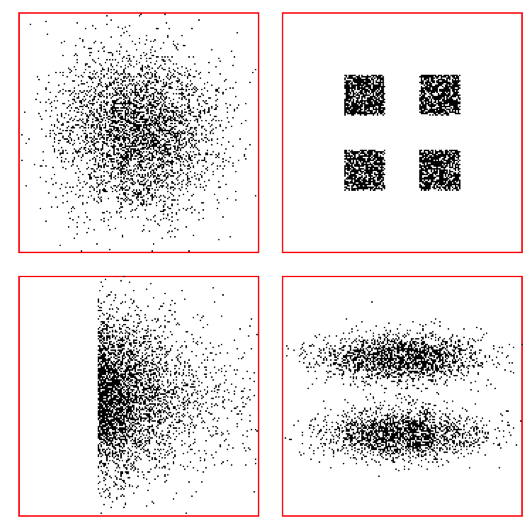
\includegraphics[scale=0.7]{img/Distribuzioni.png}
\caption{Questi quattro dataset hanno statistiche identiche, la stessa media e la stessa matrice di covarianza. }
\label{distribuzioni}
\end{figure}
In Figura \ref{distribuzioni} vengono mostrati quattro dataset differenti che hanno la stessa media e la stessa matrice di covarianza. Ovviamente, le statistiche del secondo ordine non sono in grado di rilevare tutta la struttura dei dati. Se assumiamo che i campioni sono distribuiti secondo una mixtura di $c$ distribuzioni normali, allora possiamo approssimare una grande varietà di situazioni. Ciò significa assumere che i campioni sono rappresentati da una nuvola dalla forma di una ellissoide di varie grandezze e direzioni. Se il numero delle componenti è sufficientemente alto, possiamo approssimare virtualmente qualsiasi distribuzione come mixtura ed usare i parametri della mixtura per descrivere i dati. Purtroppo abbiamo visto che la stima dei parametri di una mixtura non è un problema abbastanza semplice, un altrenativa sarebbe quella di usare una tecnica non parametrica descritta nel capitolo \ref{metodinonparametrici} per stimare le densità di mixture non conosciute, che se accurata, il risultato della stima è certamente una completa descrizione di cosa possiamo apprendere dai dati. Le regioni di alta densità, le quali potrebbero corrispondere a significanti sottoclassi della popolazione, possono essere trovate osservando i picchi della densità stimata.\\

\noindent Se invece l'obiettivo è quello di trovare le sottoclassi, allora una alternativa più diretta è quella di usare la procedura di \emph{clustering}. In breve, la procedura di clusterind produce una descrizione dei dati in termini di gruppi (cluster) di punti che posseggono una forte similarietà. La procedura di clustering formale usa una funzione criterio, come la somma della radice quadrate delle distanze dal centroide. 

\subsection{Similarity Measures}
Una volta descritto il problema di clustering come la procedura intenta a trovare raggruppamtenti  naturali in un insieme di dati, siamo obbligati a definire cosa intendiamo per raggruppamento naturale. Per quale motivo possiamo dire che i campioni di un cluster sono più simili tra loro rispetto a quelli di un altro cluster? Queste domande portano a die problemi separati:
\begin{itemize}
\item Come si dovrebbe misurare la similarietà tra i campioni?
\item Come si dovrebbe valutare il partizionamento di un insieme di campioni in clusters?
\end{itemize}
In questa sezione di occupiamo del primo dei due problemi.\\

\noindent La più importante misura di similarietà tra due campioni è la distanza fra loro. Un modo per incominciare l'investigazione è quello di definire una metrica di riferimento adeguata e calcolare la matrice delle distanze tra tutte le coppie di campioni. Se la distanza è una buona misura di dissimilarietà allora dobbiamo aspettarci che la distanza tra i campioni dello stesso cluster è significativamente minore rispetto alla distanza di campioni appartenenti a cluster differenti. Supponiamo per un momento che la distanza euclidea fra due campioni dello stesso cluster deve essere minore di una soglia che indichiamo con $d_0$, è ovvio che la scelta di $d_0$ è molto importante, se $d_0$ è molto grande, allora tutti i campioni verranno assegnati ad un solo cluster, viceversa, se $d_0$ è molto piccolo ogni campione resterà isolato. Per ottenere u raggruppamento naturale, $d_0$ dovrà essere maggiore della distanza intra-cluster (\emph{within cluster}) e minore della distanza fra cluster (\emph{between-cluster})(Fig.\ref{similarieta}).\\
 
\begin{figure}
\centering
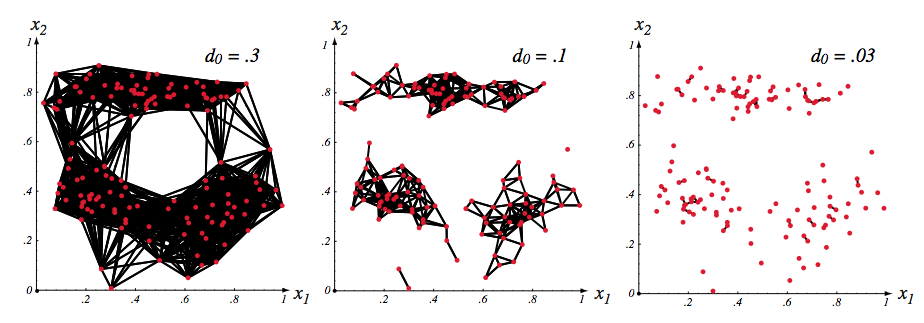
\includegraphics[scale=0.45]{img/similarieta.png}
\caption{Esempio di clustering basato sulla distanza come misura di similarietà}
\label{similarieta}
\end{figure}

\noindent Meno evidente è forse il fatto che i risultati del clustering dipendono dalla scelta di una distanza euclidea come misura di dissimilarietà. Questa particolare scelta è giustificata se lo spazio delle caratteristiche è isotropico ed i dati sono distribuiti uniformemente lungo tutte le direzioni, i cluster definiti secondo questo criterio sono invarianti per traslazione o rotazione. Invece non sono invarianti a trasformazioni lineari oppure a trasformazioni che distorciono le relazioni di distanza. 
\begin{figure}
\centering
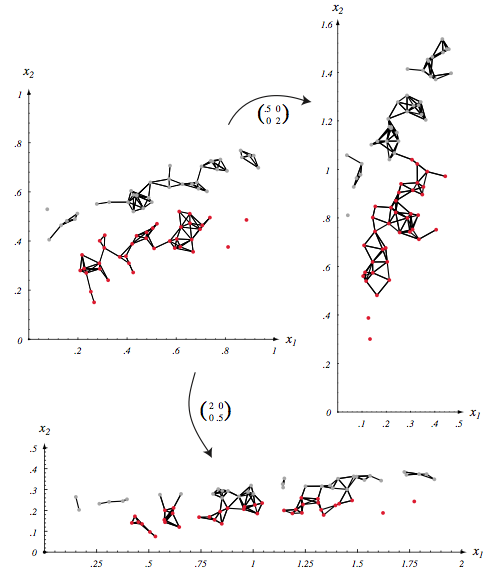
\includegraphics[scale=0.8]{img/similarieta1.png}
\caption{}
\label{similarieta1}
\end{figure}
In figura \ref{similarieta1} c'è un esempio di scaling degli assi, possiamo osservare i differenti raggruppamenti dei dati. Un modo per ottenere l'invarianza è quello di normalizzare i dati. Per esempio, per ottenere l'invarianza per lo spostamento o scaling degli assi si potrebbe traslare e scalare gli assi in modo tale da standardizzare i dati, quindi con media zero e varianza unitaria. Invece per ottenere l'invarianza per rotazione un metodo potrebbe essere quello di ruotare gli assi in modo tale da farli coincidere con gli autovettori della matrice di covarianza. Un alternativa allo scaling degli assi invece potrebbe essere quella di considerare altre metriche. Per esempio una potrebbe essere del tipo
\begin{equation}
d(\mathbf{x}, \mathbf{x}') = \left( \sum_{k=1}^d \abs{x_k - x_k'}^q \right)^{1/q} 
\end{equation}
dove $q \geq 1$ è un parametro. Impostando $q=2$ otteniamo proprio la distanza euclidea mente con $q=1$ otteniamo la distanza di \emph{Manhattan} o \emph{city block}. C'è da notare che soltanto con $q=1$ è invariante per rotazione e traslazione. Un altra alternativa è quella di usare alcuni tipi di metriche basate sui dati stessi, come la distanza di \emph{Mahalanobis}.\\

\noindent Più in generale, si potrebbe abbandonare il criterio basato sulla distanza ed introdurre un criterio basato su una funzione di similarietà $s(\mathbf{x}, \mathbf{x}')$ per paragonare i due vettori $\mathbf{x}$ ed $\mathbf{x}'$. Convenzionalmente, questa è una funzione simmetrica i cui valori sono grandi quando i due vettori sono simili. Per esempio l'angolo tra i due vettori è un importante misura della loro similarietà, quindi la normalizzazione del prodotto interno
\begin{equation}\label{50}
s(\mathbf{x}, \mathbf{x}') = \frac{\mathbf{x}^t\mathbf{x}'}{\norma{\mathbf{x}} \norma{\mathbf{x}'}}
\end{equation}
potrebbe essere un appropriata funzione di similarietà. Questa misura, che è il coseno dell'angolo tra i due vettori, è invariante per rotazione e dilatazione nonstante non sia invariante per traslazione e per le trasformazioni lineari in generale. \\

\noindent Quando le caratteristiche sono valori binari (0 o 1) la funzione di similarietà (Eq. \ref{50}) ha una semplice intrepretazione in termini di caratteristiche condivise. Diciamo che un campione $\mathbf{x}$ possiede l' \emph{i}-esimo attributo se $x_i=1$. Allora $\mathbf{x}^t\mathbf{x}'$ è semplicemente il numero di attributi posseduti da $\mathbf{x}$ e $\mathbf{x}'$, e $\norma{\mathbf{x}} \norma{\mathbf{x}'} = (\mathbf{x}^t \mathbf{xx}'^t \mathbf{x}')^{1/2}$ è la media geometrica del numero di attributi posseduti da $\mathbf{x}$ e da $\mathbf{x}'$. Così, $s(\mathbf{x}, \mathbf{x}')$ è una misura relativa agli attributi posseduti in comune. Alcune semplici variazioni sono
\begin{equation}
s(\mathbf{x}, \mathbf{x}') = \frac{\mathbf{x}^t \mathbf{x}'}{d}
\end{equation}
che sono gli attributi condivisi, e
\begin{equation}
s(\mathbf{x}, \mathbf{x}') = \frac{\mathbf{x}^t \mathbf{x}'}{\mathbf{x}^t \mathbf{x} + \mathbf{x}'^t \mathbf{x}' - \mathbf{x}^t \mathbf{x}'} 
\end{equation}
che è il rapporto tra il numero di attributi condivisi ed il numero di attributi posseduti da $\mathbf{x}$ o da $\mathbf{x}'$. Questa misura è nota come distanza di Tanimoto ed è frequentemente incontrata nel campo di \emph{information retrival}.
 
\section{Criterion Functions For Clustering}
Abbiamo appena considerato il primo dei problemi del clustering cioè quello di come misurare la similarietà. Adesso ci occuperemo del secondo problema quindi una funzione criterio che deve essere ottimizzata. Supponiamo che abbiamo un insieme $\mathcal{D}  = { \mathbf{x}_1, \dots, \mathbf{x}_n }$ di $n$ campioni che devono essere partizionati in $c$ sottoinsimemi $\mathcal{D}_1, \dots, \mathcal{D}_c$. Ogni sottoinsieme rappresenta un cluster, ed i campioni appartenenti allo stesso cluster sono in qualche modo più simili tra loro rispetto agli altri cluster. Un modo per fare questo è quello di definire una funzione criterio che misura la qualità del clustering. Allora il problema è quello di trovare la partizione che estremizza la funzione criterio.

\subsection{The Sum-of-Squared-Error Criterion}
La funzione criterio più semplice e quella maggiormente usata per il clustering è il \emph{sum-of-squared-error}. Denotiamo con $n_i$ i numero di campioni nei sottoinsimemi $\mathcal{D}_i$ e denotiamo con $\mathbf{m}_i$ le medie di questi campioni, 
\begin{equation}
\mathbf{m}_i = \frac{1}{n_i} \sum_{x \in \mathcal{D}_i} \mathbf{x}
\end{equation}
Allora la \emph{sum-of-squared-error} è definita mediante la seguente formula
\begin{equation}
J_e = \sum_{i=1}^c \sum_{x \in \mathcal{D}_i} \norma{\mathbf{x} - \mathbf{m}_i}^2
\end{equation}
Questa funzione criterio ha una semplice interpretazione: Dati i cluster $\mathcal{D}_i$, il vettore media $\mathbf{m}_i$ è quello che meglio rappresenta i campioni in $\mathcal{D}_i$ nel senso che minimizza la somma delle radici quadrate della distanza $\mathbf{x}-\mathbf{m}_i$. Così, $J_e$ misura l'errore totale rappresentato dagli $n$ campioni $\mathbf{x}_1, \dots, \mathbf{x}_n$ raggruppati in $c$ cluster con centroidi $\mathbf{m}_1, \dots, \mathbf{m}_c$. Il valore di $J_e$ dipende da come i campioni sono raggruppati in cluster e dal numero di cluster. La partizione ottima è definita quando $J_e$ è minimo, clustering di questi tipo sono spesso chiamati partizioni a minima varianza, si potrebbe andare incontro a problemi quando tra i cluster c'è una grande differenza in base al numero di campioni, in questo caso può succedere che potrebbero esserci problemi nella partizione come  mostra la figura \ref{cluster}.
\begin{figure}
\centering
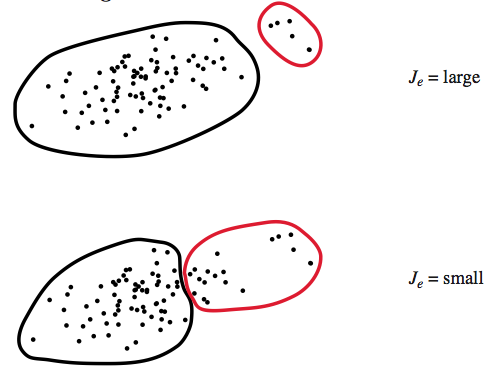
\includegraphics[scale=0.5]{img/cluster.png}
\caption{}
\label{cluster}
\end{figure}
 
\section{Iterative Optimization}
Una volta che la funzione criterio è stata selezionata, il clustering diventa un problema ben definito come ottimizzazione discreta: Trovare le partizioni di un insieme di campioni che estremizzano la funzione criterio. Poichè l'insieme dei campioni è finito, ci sono quindi soltanto un numero finito di partizioni, così, il problema può essere sempre risolto con una enumerazione esaustiva, ma la complessità computazionale di un algoritmo rende tale approccio impensabile. Ci sono approssimativamente $c^n /c!$ modi di partizionare un insieme di $n$ elementi in $c$ sottoinsiemi, ed il fatto che dipende esponenziamente da $n$ è schiacciante. Per esempio una ricerca esaustiva del partizionamento di 100 campioni in 5 cluster richiede più di $10^{67}$ partizionamenti. \\

\noindent L'approccio più frequentemente usato nel cercare un partizionamento ottimo è un ottimizzazione iterativa. L'idea di base è quella di trovare delle partizioni iniziali e muovere i campioni da un gruppo all'altro in modo tale da migliorare i valori della funzione criterio.  In genere questi approcci garantiscono un ottimizzazione locale ma non globale, inoltre c'è da considerare che differenti punti di inizio portano a soluzioni differenti e non si può mai sapere se è stata trovata la migliore soluzione. Nonostante queste limitazioni, il fatto che la complessità computazionale è sopportabile fa di esso un approccio attrattivo.\\

\noindent Consideriamo l'uso di un miglioramento iterativo per minimizzare il criterio \emph{sum-of-squared-error} $J_e$, scritto come
\begin{equation}
J_e = \sum_{i=1}^c J_i
\end{equation}
dove l'errore effettivo per cluster è definito nel seguente modo
\begin{equation}
J_i = \sum_{\mathbf{x} \in \mathcal{D}_i} \norma{\mathbf{x}-\mathbf{m}_i}^2
\end{equation}
e la media di ogni cluster è come prima
\begin{equation}
\mathbf{m}_i = \frac{1}{n_i} \sum_{\mathbf{x} \in \mathcal{D}} \mathbf{x}
\end{equation}
Supponiamo che il campione $\hat{\mathbf{x}}$ è attualmente nel cluster $\mathcal{D}_i$ e si tenta di spostarlo nel cluster $\mathcal{D}_j$. Allora $\mathbf{m}_j$ cambia
\begin{equation}
\mathbf{m}_j^* = \mathbf{m}_j + \frac{\hat{\mathbf{x}}-\mathbf{m}_j}{n_j+1}
\end{equation}
e $J_j$ si incrementa
\begin{equation}
J_j^* = \sum_{\mathbf{x} \in \mathcal{D}_j} \norma{\mathbf{x} - \mathbf{m}_j^*}^2 + \norma{\hat{\mathbf{x}} - \mathbf{m}_j^*}^2
\end{equation}
effettuando gli opportuni calcoli
\begin{equation}
\begin{split}
J_j^* &= \sum_{\mathbf{x} \in \mathcal{D}_j} \norma{\mathbf{x} - \mathbf{m}_j^*}^2 + \norma{\hat{\mathbf{x}} - \mathbf{m}_j^*}^2\\
&= \left(  \sum_{\mathbf{x} \in \mathcal{D}_i} \left|\left| \mathbf{x} - \mathbf{m}_j - \frac{\hat{\mathbf{x}}-\mathbf{m}_j}{n_j+1} \right| \right|^2   \right) + \left| \left|  \frac{n_j}{n_j +1} (\hat{\mathbf{x}} - \mathbf{m}_j)  \right| \right|^2 \\
&= J_j + \frac{n_j}{n_j+1}\norma{\hat{\mathbf{x}} - \mathbf{m}_j}^2
\end{split}
\end{equation}
Sotto l'assunzione che se $n_i \neq 1$ allora $\mathbf{m}_i$ cambia in
\begin{equation}
\mathbf{m}_i^* = \mathbf{m}_i - \frac{\hat{\mathbf{x}} - \mathbf{m}_i }{n_j-1}
\end{equation}
e $J_i$ si decrementa 
\begin{equation}
J_i^* = J_i - \frac{n_i}{n_i-1} \norma{\hat{\mathbf{x}} - \mathbf{m}_i}^2
\end{equation}
Queste equazioni semplificano notevolmente il calcolo delle variazioni nella funzione criterio. Spostare $\hat{\mathbf{x}}$ da $\mathcal{D}_i \ \text{a} \ \mathcal{D}_j$ è un vantaggio se il decremento i $J_i$ è maggiore dell'incremento in $J_j$. Questo il caso in cui
\begin{equation}
\frac{n_i}{n_i-1} \norma{\hat{\mathbf{x}} - \mathbf{m}_i}^2 > \frac{n_j}{n_j+1} \norma{\hat{\mathbf{x}} -\mathbf{m}_j }^2
\end{equation}
il che tipicamente succede quando $\hat{\mathbf{x}}$ è più vicino ad $\mathbf{m}_j$ che ad $\mathbf{m}_i$. Se il riassegnamento è redditizio, allora il maggiore decremento della somma degli errori al quadrato è ottenuto selezionando il cluster per il quale $n_j \norma{\hat{\mathbf{x}} - \mathbf{m}_j}^2/(n_j+1)$ è minimo. Questo posta alla seguente procedura di clustering:

\begin{codebox}
\Procname{$\proc{Basic Iterative Minimum-Squared-Error Clustering}$}
\li \textbf{begin initialize} $n, c, \mathbf{m}_1, \mathbf{m}_2, \dots, \mathbf{m}_c$
\li 	\Do seleziona casualmente il campione $\hat{\mathbf{x}}$
\li		$i \gets \arg \min{i} \norma{\mathbf{m}_{i'}- \hat{\mathbf{x}} }$
\li	\If $n_i \neq 1$	
\li 		\Then calcola
\li              
		$\rho_j=
		\begin{cases}
		\frac{n_i}{n_i+1} \norma{\hat{\mathbf{x}} - \mathbf{m}_i}^2 & \ \ \ \ \ j \neq i\\
		\frac{n_i}{n_i-1} \norma{\hat{\mathbf{x}} - \mathbf{m}_i}^2 &  \ \ \ \ \ i = j 
		\end{cases}$ 		
\li		\If $\rho_k \leq \rho_j  \ \text{per ogni} \ j$
\li			\Then trasferisci $\hat{\mathbf{x}} \ \text{in} \ \mathcal{D}_k$
\li				 ricalola $J_e, \mathbf{m}_i, \mathbf{m}_k$
		\End 
\li	\Until non si ha nessun cambiamenti di $J_i$ in $n$ tentativi	
	\li \Return $\mathbf{m}_1, \mathbf{m}_2, \dots, \mathbf{m}_c$	
	\End
	\End
\li \textbf{end}	
\end{codebox}
Questa procedura è essenzialmente una versione sequenziale della procedura $k$-means descritta nella sezione precedente. Nel caso del $k$-means si aspettava finchè tutti gli $n$ campioni venivano classificati prima dell'aggiornamento, mentre la procedura Iterativa Minimum-Squared-Error aggiorna dopo che ogni campione è stato riclassificato. Questa è una procedura graduale ottimale e può essere facilmente modificata per applicarla  a problemi nei quali i campioni sono acquisiti sequenzialmente e quindi il clustering potrebbe essere fatto in modo \emph{on-line}.   

\section{Hierarchical Clustering}


\subsection{Definitions}
Consideriamo di voler partizionare $n$ campioni in $c$ cluster. Se incominciamo con $n$ cluster allora ogni cluster è formato da un unico campione. La prossima partizione la effettuiamo in $n-1$ cluster, poi ancora in $n-2$ e così via, finchè tutti i campioni formino un unico cluster. Si può affermare che siamo al livello $k$ della sequenza quando $c = n-k+1$.  Così facendo, il livello uno corrisponde ad $n$ cluster ed il livello $n$ corrisponde ad un unico cluster. Dati due campioni $\mathbf{x}$ e $\mathbf{x}'$ situati allo stesso livello allora potranno essere raggruppati insieme nello stesso cluster. Se questo processo ha la propietà che se due campioni appartengono allo stesso cluster al livello $k$ e rimangono insieme per tutti i livelli più alti, allora questo processo è detto \emph{hierarchical clustering} (clustering gerarchico).\\

\noindent La più naturale rappresentazione del clustering gerarchico è un albero chiamato dendogramma, il quale mostra come i campioni sono stati raggruppati. 
\begin{figure}
\centering
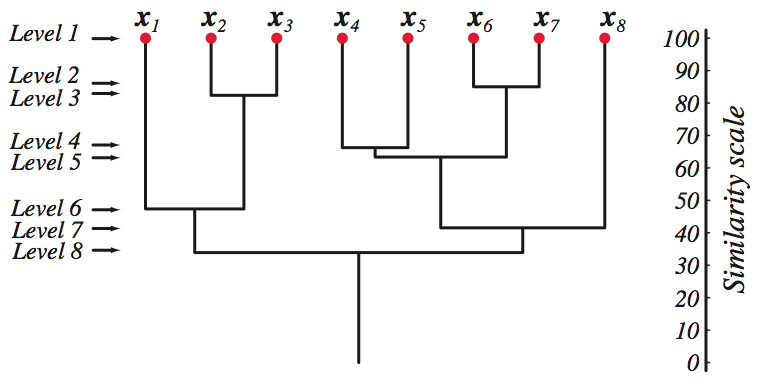
\includegraphics[scale=0.5]{img/dendogramma.png}
\caption{Esempio di dendogramma}
\label{dendogramma}
\end{figure}
In figura \ref{dendogramma} è stato mostrato un dendogramma per un problema semplice con otto campioni. Al livello $k=1$ ogni singolo campione rappresenta un cluster. Al livello $k=2$, $\mathbf{x}_6$ ed $\mathbf{x}_7$ sono stati raggruppati in un cluster e staranno insieme nello stesso cluster fino alla fine. Se è possibile misurare delle similarietà tra i cluster allora il dendogramma è generalmente disegnata con un scala che indica la similarietà tra i cluster che sono stati raggruppati.\\

\noindent Ci sono anche altre rappresentazioni del clustering gerarchico, come l'uso degli insiemi e quindi dei diagrammi di Venn oppure una rappresentazione utilizzando le parentesi graffe per indicare gli insiemi. Ma il dendogramma resta sempre il metodo preferito.\\

\noindent Data la sua semplicità, il clustering gerarchico è una tecnica molto usata nel metodo \emph{unsupervised}. La stessa procedura, inoltre può essere divisa in due distinti approcci. L'approccio Agglomerativo (bottom-up), questa procedura inizia da $n$ cluster composti da un sono campione e poi effettua una fusione tra cluster. L'altro approccio definito $\emph{Divisive}$ è top-down, ed è l'inverso del precedente, quindi si parte da un unico cluster per poi dividere in cluster più piccoli. 

\subsection{Agglomerative Hierarchical Clustering}
I passi più importanti della procedura agglomerativa sono contenuti nel seguente algoritmo, dove $c$ è il numero di cluster finale
\begin{codebox}
\Procname{$\proc{Agglomerative Hierarchical Clustering}$}
\li \textbf{begin initialize} $c, \hat{c} \gets n, \mathcal{D}_i \gets \{ \mathbf{x}_i \}, i=1,\dots, n$
\li	\Do $\hat{c} \gets \hat{c} - 1$
\li		trova il cluster più vicino, $\mathcal{D}_i \ \text{e} \ \mathcal{D}_j$
\li		fondi $\mathcal{D}_i$ e $\mathcal{D}_j$
	\End
\li	\Until	 $c=\hat{c}$
\li	\Return $c$ clusters
\li \textbf{end}	
\end{codebox}
Come descritto sopra, qeusta procedura termina quando è stato ottenuto il numero di cluster specificato. Se si continua fino a $c=1$ allora si ottiene proprio il dendogramma. A qualsiasi livello la distanza tra i cluster più vicini può fornire il valore di dissimilarietà a quel livello. Da notare che non è stata introdotta come viene misurata la distanza tra clusters ed è interessata la linea $3$ dell'algoritmo. Le considerazioni sono molto simili alle funzioni criterio utilizzate nel criterio generale. Per semplicità focalizziamo l'attenzione sulle seguenti misure di distanza
\begin{gather}
d_{min}(\mathcal{D}_i, \mathcal{D}_j) = \min_{\mathbf{x} \in \mathcal{D}_i, \mathbf{x}' \in \mathcal{D}_j} \norma{\mathbf{x} - \mathbf{x}'}\\
d_{max}(\mathcal{D}_i, \mathcal{D}_j) = \max_{\mathbf{x} \in \mathcal{D}_i, \mathbf{x}' \in \mathcal{D}_j} \norma{\mathbf{x} - \mathbf{x}'} \\
d_{avg}(\mathcal{D}_i, \mathcal{D}_j) = \frac{1}{n_i n_j} \sum_{\mathbf{x} \in \mathcal{D}_i} \sum_{\mathbf{x}' \in \mathcal{D}_j} \norma{\mathbf{x} - \mathbf{x}'}\\
d_{mean}(\mathcal{D}_i, \mathcal{D}_j) = \norma{\mathbf{m}_i - \mathbf{m}_j}  
\end{gather}
Queste misure di similarietà generalmente producono cluster compatti e ben separati.

\paragraph{Nearest-Neighbor Algorithm}
Quando viene usata la funzione $d_{min}(\cdot, \cdot)$ per misurare la distanza tra cluster allora l'algoritmo prende il nome di \emph{Nearest-Neighbor Algorithm} o \emph{minimum algorithm}. Inoltre se l'algoritmo è terminato quando la distanza tra  cluster più vicini eccede un' arbitraria soglia allora è chiamato \emph{single-linkage algorithm}. Supponiamo di immaginare i campioni come nodi di un grafo, con gli \emph{edges} che formano un cammino tra i nodi nello stesso sottoinsieme $\mathcal{D}_i$. Quando viene usata la misura di distanza $d_{min}(\cdot, \cdot)$ la fusione tra $	\mathcal{D}_i$ e $	\mathcal{D}_j$ corrisponde nell'aggiungere un \emph{edge} tra la coppia di nodi più vicina in  $	\mathcal{D}_i$ e $	\mathcal{D}_j$. Poiché il collegamento  avviene sempre tra cluster differenti allora il grafo risultante non è mai un circuito chiuso, ma questa procedura genera un albero. Se invece si continua finché tutti i sottoinsiemi sono connessi allora il risultato è uno \emph{spanning tree}, un albero con un cammino da e verso qualsiasi nodo. Così utilizzando $d_{min}(\cdot, \cdot)$ come distanza di misura, allora la procedura di clustering agglomerativa diventa un algortirmo per generare un \emph{minimal spanning tree}.   
\begin{figure}
\centering
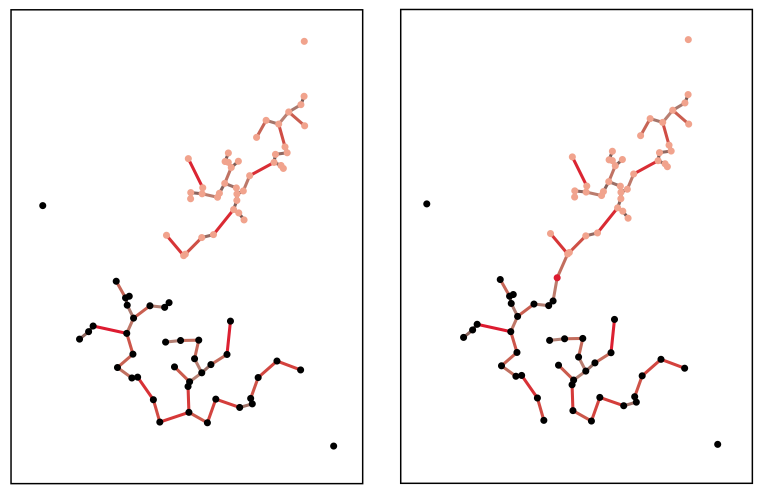
\includegraphics[scale=0.5]{img/spanningtree.png}
\caption{}
\label{spanning}
\end{figure}
In Figura \ref{spanning} sono mostrati i risultati applicando la procedura a dei dati gaussiani. In entrambi i casi la procedura è stata fermata ottenendo così due grandi cluster. Il \emph{minimal spanning tree} può essere ottenuto aggiungendo  l' edge più corto possibile tra i due cluster.

\paragraph{The Farthest-Neighbor Algorithm}
Quando come misura della distanza viene utilizzata $d_{max}(\cdot, \cdot)$ allora l'algoritmo è chiamato \emph{Farthest-Neighbor Algorithm} o \emph{maximum algorithm}. Invece se termina quando la distanza tra i cluster più vicini eccede una soglia arbitraria allora è detto \emph{complete-linkage algorithm}. La procedura può essere vista come la generazione di un grafo nel quale gli edge collegano tutti i nodi di un clsuter. Nella terminologia della teoria dei grafi, ogni cluster costituisce un sottografo completo. La distanza tra due cluster è determinata mediante la più grande distanza tra nodi di due cluster. Quando i cluster più vicini vengono uniti allora il grafo cambia aggiungendo lati tra ogni coppia di nodi dei due cluster. 
\begin{figure}
\centering
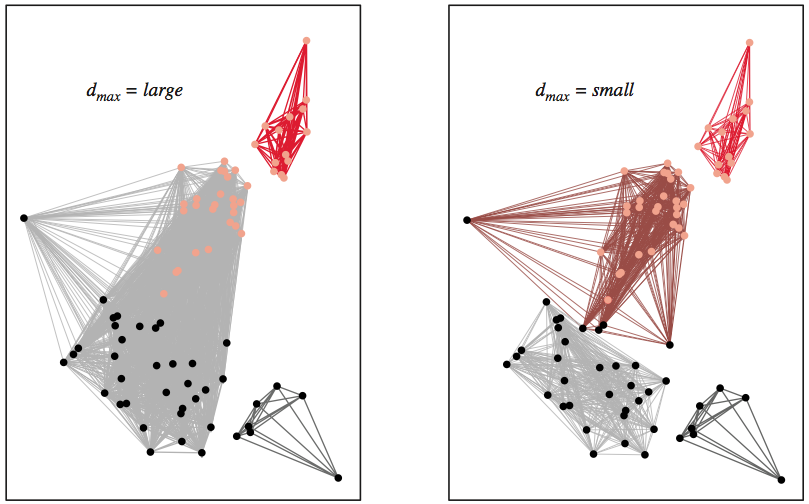
\includegraphics[scale=0.4]{img/grafo2.png}
\caption{}
\label{grafo2}
\end{figure}
In figura \ref{grafo2} è mostrata la tecnica. 

\subsection{Stepwise-Optimal Hierarchical Clustering}
Si specifica il numero di cluster, si pone ogni pattern in un cluster e si ripeteno
\subsection{da completare}

%
